\documentclass[11pt,a4paper]{article}
\usepackage{nabiadoc}
\usepackage{tikz}
\usetikzlibrary{positioning,arrows.meta,fit,calc}
\usepackage{caption}
\captionsetup[lstlisting]{justification=raggedright, singlelinecheck=false, font=small, labelfont=bf}
\usepackage{tabularx}

% Generated at build time by extract_snippets.py: excerpt locations, the MCP
% tool catalogue (tools.tex) and the AI configuration fields (config.tex).
\input{snippets.tex}
\newcommand{\snippetsource}[1]{\csname snippet@#1\endcsname}
\newcommand{\snippet}[3]{%
  \lstinputlisting[language=#2, caption={#3\\{\footnotesize\ttfamily\snippetsource{#1}}}]{#1.txt}}
% A prompt: plain text, wrapped.
\newcommand{\prompt}[2]{%
  \lstinputlisting[language={}, basicstyle=\ttfamily\scriptsize, keywordstyle={}, commentstyle={},
                   caption={#2\\{\footnotesize\ttfamily\snippetsource{#1}}}]{#1.txt}}
\lstset{basicstyle=\ttfamily\scriptsize, captionpos=t, numbers=none, aboveskip=8pt, belowskip=8pt,
        tabsize=4, keepspaces=true, breaklines=true, postbreak=\mbox{\textcolor{gray}{$\hookrightarrow$}\space}}
\renewcommand{\lstlistingname}{Code}
\newcommand{\sth}{\mathcal{S}}  % soft thresholding

% Pointers from a concept to its code.
\newcommand{\coderef}[1]{{\footnotesize\texttt{\snippetsource{#1}}}}
\newenvironment{codepointers}{%
  \par\smallskip\begingroup\footnotesize\noindent\textcolor{blue!50!black}{\textbf{Code}}\par\nopagebreak
  \begin{list}{}{\setlength{\leftmargin}{1.2em}\setlength{\itemsep}{0pt}\setlength{\parsep}{0pt}\setlength{\topsep}{1pt}}}%
  {\end{list}\endgroup\smallskip}
\newcommand{\codeitem}[2]{\item #2 --- \texttt{\snippetsource{#1}}}

% MCP tool catalogue entries (tools.tex).
\newcommand{\toolentry}[3]{\subsubsection*{\texttt{#1}}\vspace{-0.6em}
  \noindent{\footnotesize\textcolor{gray!30!black}{\emph{#2}\hfill\texttt{#3}}}\par\smallskip}
\newcommand{\modelentry}[2]{\subsubsection*{Input schema \texttt{#1}}\vspace{-0.6em}
  \noindent{\footnotesize\textcolor{gray!30!black}{\emph{pydantic model}\hfill\texttt{#2}}}\par\smallskip}
\newenvironment{toolparams}{\begin{description}\footnotesize\setlength{\itemsep}{0pt}\setlength{\parsep}{0pt}}{\end{description}}
% A reference to a section of another project's document.
\newcommand{\xref}[2]{\emph{#2} (#1 reference)}

\title{nabia C++: Methods and Reference\\[0.3em]
\large The numerical library, its command-line application and its Python bindings}
\author{nabia documentation}
\date{October 2026}

\begin{document}
\maketitle

\begin{abstract}
This document is the reference for the C++ project of nabia (\code{cpp/}). It describes
every method the library implements, stated mathematically, with proofs where a property is
relied on:
\begin{itemize}
  \item time series containers, signal filters, forecasters (exponential smoothing, Kalman
        filter, Gaussian processes) and five optimizers;
  \item risk measures, risk budgeting, the walk-forward portfolio engine and its metrics;
  \item the elastic net factor regression engine;
  \item the command-line application, and the pybind11 bindings that build the
        \code{nabia\_python\_bridge} wheel for every Python version and platform.
\end{itemize}
The Python package built on the wheel and the web application with its agents have their own
references (\code{python/doc} and \code{webui/doc}). Each concept points to the code that
implements it, by file and line range, and the key code is shown in excerpts \emph{extracted
from the source when the document is built}, so a renamed function stops the build instead of
leaving a stale reference.
\end{abstract}

\tableofcontents
\clearpage
%==============================================================================
\part{Overview}

\section{Purpose}
nabia is a platform for researching and running \emph{systematic trend strategies} across
equity indices, government bond futures, commodities and crypto. The C++ library is its
numerical core: it extracts trends from noisy prices (\S\ref{sec:signal}, \S\ref{sec:forecast}),
turns risk budgets into positions with a deterministic, tested engine (\S\ref{sec:riskbudgeting},
\S\ref{sec:engine}), measures the result (\S\ref{sec:metrics}) and explains a target series with
factors (\S\ref{sec:regression}). Everything is available to Python through the
\code{nabia\_python\_bridge} wheel (\S\ref{sec:bridge}).

\section{Architecture}\label{sec:architecture}
\begin{figure}[ht]
\centering
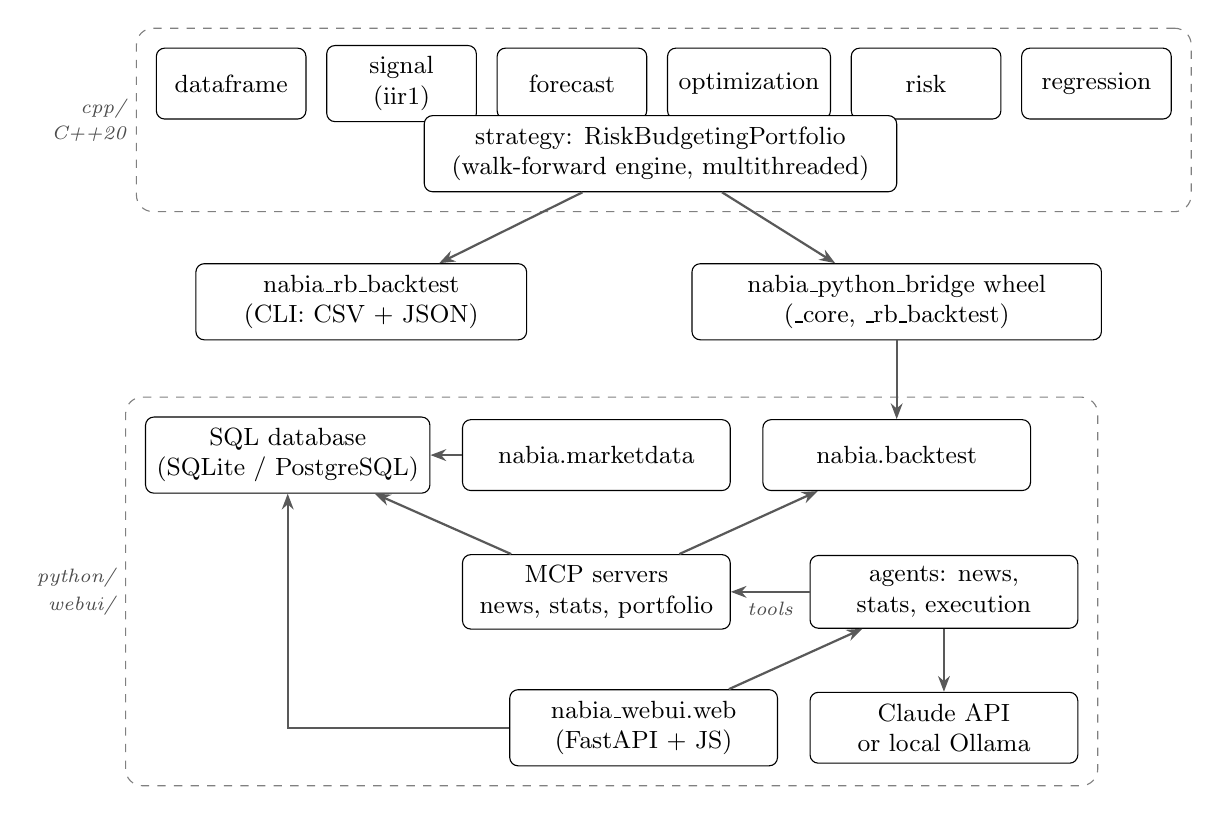
\begin{tikzpicture}[
  box/.style={draw, rounded corners=3pt, align=center, minimum height=9mm, font=\small, fill=white, inner sep=4pt},
  layer/.style={draw, dashed, rounded corners=6pt, inner sep=7pt, gray},
  arrow/.style={-{Stealth[length=2mm]}, thick, gray!70!black},
  lbl/.style={font=\scriptsize\itshape, gray!60!black}]
  \node[box, minimum width=19mm] (df) {dataframe};
  \node[box, right=2.5mm of df, minimum width=19mm] (sig) {signal\\(iir1)};
  \node[box, right=2.5mm of sig, minimum width=19mm] (fc) {forecast};
  \node[box, right=2.5mm of fc, minimum width=19mm] (opt) {optimization};
  \node[box, right=2.5mm of opt, minimum width=19mm] (risk) {risk};
  \node[box, right=2.5mm of risk, minimum width=19mm] (reg) {regression};
  \node[box, below=4mm of $(fc)!0.5!(opt)$, minimum width=60mm] (strat) {strategy: RiskBudgetingPortfolio\\(walk-forward engine, multithreaded)};
  \node[layer, fit=(df)(reg)(strat), label={[lbl]left:\shortstack[r]{cpp/\\C++20}}] (core) {};
  \node[box, below=9mm of strat, xshift=-38mm, minimum width=42mm] (cli) {nabia\_rb\_backtest\\(CLI: CSV + JSON)};
  \node[box, below=9mm of strat, xshift=30mm, minimum width=52mm] (bind) {nabia\_python\_bridge wheel\\(\_core, \_rb\_backtest)};
  \node[box, below=10mm of bind, minimum width=34mm] (pf) {nabia.backtest};
  \node[box, left=4mm of pf, minimum width=34mm] (md) {nabia.marketdata};
  \node[box, left=4mm of md, minimum width=30mm] (db) {SQL database\\(SQLite / PostgreSQL)};
  \node[box, below=8mm of md, minimum width=34mm] (mcp) {MCP servers\\news, stats, portfolio};
  \node[box, right=10mm of mcp, minimum width=34mm] (agents) {agents: news,\\stats, execution};
  \node[box, below=8mm of agents, minimum width=34mm] (llm) {Claude API\\or local Ollama};
  \node[box, left=4mm of llm, minimum width=34mm] (web) {nabia\_webui.web\\(FastAPI + JS)};
  \node[layer, fit=(db)(pf)(mcp)(agents)(llm)(web), label={[lbl]left:\shortstack[r]{python/\\webui/}}] (py) {};
  \draw[arrow] (strat) -- (cli);
  \draw[arrow] (strat) -- (bind);
  \draw[arrow] (bind) -- (pf);
  \draw[arrow] (md) -- (db);
  \draw[arrow] (mcp) -- (db);
  \draw[arrow] (mcp) -- (pf);
  \draw[arrow] (agents) -- node[lbl, below]{tools} (mcp);
  \draw[arrow] (agents) -- (llm);
  \draw[arrow] (web) -- (agents);
  \draw[arrow] (web.west) -| (db.south);
\end{tikzpicture}
\caption{The whole system and its three projects. Arrows point from a component to what it uses.}
\label{fig:architecture}
\end{figure}
\subsection{Three projects}
The repository holds three independent projects. Each opens on its own in an IDE, and each
has its own documentation in a \code{doc} folder:
\begin{center}\small
\begin{tabularx}{\linewidth}{@{}l l X@{}}
\toprule
Folder & IDE & Contents \\
\midrule
\code{cpp/} & CLion (CMake) & the C++ library (\code{include}, \code{src}), its tests, the
  command-line application, and the pybind11 bindings that build the
  \code{nabia\_python\_bridge} wheel into \code{dist/} \\
\code{python/} & PyCharm & the \code{nabia} package (backtests, analytics, market data) on top of
  the wheel, the examples, and the Python tests including the bridge tests \\
\code{webui/} & PyCharm & \code{nabia\_webui}: the agents, their MCP servers and the web app, on
  top of the \code{nabia} package \\
\bottomrule
\end{tabularx}
\end{center}
The projects depend on each other only through installed packages: \code{cpp} builds the wheel,
\code{python} installs it (\code{python/scripts/setup\_env.sh}), and \code{webui} installs both the
wheel and \code{python} in editable mode (\code{webui/scripts/setup\_env.sh}). Shared data, the market
database \code{data/market.db}, is at the repository root.

\subsection{Layers of the C++ project}
\begin{description}
  \item[Library] (\code{include/nabia}, \code{src}): the static library \code{nabia::nabia},
        built with CMake. It uses C++20, Eigen for linear algebra and iir1 for filter
        design. Each module exposes an abstract interface whose parameter struct is owned
        through \code{std::unique\_ptr}:
        \begin{itemize}
          \item \code{IFilter<P>} (\coderef{ifilter});
          \item \code{IForecaster<P>} (\coderef{iforecaster});
          \item \code{IOptimizer<P,R>} (\coderef{ioptimizer});
          \item \code{IRiskMeasure} (\coderef{irisk}).
        \end{itemize}
  \item[Application] \code{nabia\_rb\_backtest} (\code{apps/rb\_backtest}): a backtest from a
        prices CSV and a JSON configuration, written to CSV (\S\ref{sec:cli}).
  \item[Python bindings] (\code{bindings}): two pybind11 modules in one package,
        \code{nabia\_python\_bridge}. \code{\_core} exposes the whole library (\S\ref{sec:bridge});
        \code{\_rb\_backtest} exposes the JSON-configured backtest of the application
        (\S\ref{sec:rbbindings}). \code{pyproject.toml} builds them into a wheel (\S\ref{sec:wheels}).
\end{description}

\subsection{Directory map}
\begin{center}\small
\begin{tabular}{@{}l>{\raggedright\arraybackslash}p{10cm}@{}}
\toprule
Path (in \code{cpp/}) & Contents \\
\midrule
\code{include/nabia/dataframe} & \code{TimeSeries}, \code{DataFrame}, the \code{TimeIndex} concept \\
\code{include/nabia/signal} & \code{IFilter}, \code{EWMA}, \code{ButterworthBandPass}, smoothing helpers \\
\code{include/nabia/forecast} & \code{IForecaster}, SES, Kalman filter, Gaussian process, kernels \\
\code{include/nabia/optimization} & \code{IOptimizer}; \code{convex/}: constraints, L-BFGS, augmented Lagrangian, SQP; \code{nongradopt/}: Nelder--Mead, differential evolution \\
\code{include/nabia/risk} & \code{IRiskMeasure}, volatility, VaR, ES, \code{RiskBudgeting<Measure>} \\
\code{include/nabia/stats} & descriptive statistics, normal density, CDF and quantile \\
\code{include/nabia/strategy} & \code{RiskBudgetingPortfolio}, performance metrics \\
\code{include/nabia/regression} & \code{ElasticNet}, \code{RegressionEngine} \\
\code{src} & the implementations, in the same layout \\
\code{tests} & Catch2 unit tests \\
\code{apps/rb\_backtest} & command-line backtest (CSV and JSON) \\
\code{examples} & C++ usage examples \\
\code{bindings} & pybind11 sources (\code{src}) and the Python files of the wheel (\code{nabia\_python\_bridge}) \\
\code{pyproject.toml}, \code{scripts} & wheel build (scikit-build-core, cibuildwheel), \code{build\_wheels.sh} \\
\code{doc} & this reference and the theory notes, LaTeX sources and PDFs \\
\bottomrule
\end{tabular}
\end{center}

\subsection{Build}
Open \code{cpp/} in CLion, or use the CMake presets from that folder:
\begin{lstlisting}[language=bash]
cmake --preset debug && cmake --build --preset debug    # library, tests, app, examples, docs
ctest --preset debug                                    # the Catch2 suite and the app example
cmake --build --preset debug --target nabia_docs        # only the PDFs of doc/
\end{lstlisting}
The presets are \code{debug}, \code{release}, \code{releaseWithDebugInfo}, \code{asan} and
\code{python-bridge}; all treat warnings as errors. Dependencies are found on the system or
fetched: Eigen, iir1, Catch2, nlohmann/json and pybind11. The \code{nabia\_docs} target builds
this reference and the theory notes on exponential smoothing, the Kalman filter, Gaussian
processes, convex optimization and elastic net regression (\code{doc/<area>/*.pdf}). For this
document it first runs \code{doc/extract\_snippets.py}, which writes the excerpts and the code
locations.

%==============================================================================
\part{The numerical core (C++)}

\section{Time series containers}\label{sec:dataframe}

All numerical code works on Eigen matrices, but financial data is indexed by time.
\code{TimeSeries<Index>} and \code{DataFrame<Index>} pair an Eigen vector or matrix (rows
are times) with a \emph{strictly increasing} index:
\begin{itemize}
  \item The index type satisfies the \code{TimeIndex} concept (copyable and totally
        ordered): calendar dates, timestamps or integers.
  \item Construction validates the shapes, the ordering and unique column names.
  \item Time lookups use binary search.
\end{itemize}

\paragraph{Alignment.} Markets have different holidays. A cross-asset backtest keeps only
the dates where every asset has a finite price.

\paragraph{Returns.} Simple returns $r_t=P_t/P_{t-1}-1$ (\code{pct\_change}) or log returns
$\log(P_t/P_{t-1})$ are computed between consecutive \emph{kept} rows. A return can
therefore span a removed holiday. That is the right convention for a portfolio that can
only trade when all its markets are open.

\snippet{df_drop_missing}{C++}{Alignment: keep rows where every column is finite}
\begin{codepointers}
  \codeitem{time_index}{\code{TimeIndex} concept}
  \codeitem{timeseries}{\code{TimeSeries}}
  \codeitem{dataframe}{\code{DataFrame}}
  \codeitem{pct_change}{simple returns}
  \codeitem{log_returns}{log returns}
\end{codepointers}

\section{Signal extraction}\label{sec:signal}

Filters implement \code{IFilter<P>}. They are \emph{causal}: output $t$ uses inputs up to
$t$ only. Two modes are supported:
\begin{itemize}
  \item streaming: \code{process(x)}, one sample at a time, keeping state;
  \item batch: \code{apply(signal)}, from a fresh state, without disturbing the streaming
        state.
\end{itemize}
Filter design is delegated to iir1, behind a private implementation struct (pimpl), so iir1
never appears in public headers.

\subsection{Exponentially weighted moving average}
The EWMA is the one-pole low-pass
\[
  y_t=\alpha x_t+(1-\alpha)y_{t-1},\qquad H(z)=\frac{\alpha}{1-(1-\alpha)z^{-1}},\qquad \alpha\in(0,1].
\]
Its DC gain is $H(1)=1$, so a constant input passes unchanged.

\begin{proposition}[Seeding]
Let $\tilde y$ be the EWMA of $x_t-x_0$ started from a zero state. Then $y_t=x_0+\tilde y_t$
equals the recursion started at $y_{-1}=x_0$:
\[
  y_t=\alpha\sum_{k=0}^{t}(1-\alpha)^k x_{t-k}+(1-\alpha)^{t+1}x_0 .
\]
\end{proposition}
\begin{proof}
Unrolling the recursion from $y_{-1}$ gives
$y_t=\alpha\sum_{k=0}^{t}(1-\alpha)^kx_{t-k}+(1-\alpha)^{t+1}y_{-1}$. With a zero state,
$\tilde y_t=\alpha\sum_{k=0}^t(1-\alpha)^k(x_{t-k}-x_0)$. Using
$\alpha\sum_{k=0}^t(1-\alpha)^k=1-(1-\alpha)^{t+1}$, adding $x_0$ gives the formula with
$y_{-1}=x_0$.
\end{proof}
Starting from zero instead would bias the early outputs towards zero, so the filter seeds
with the first sample by default.

\paragraph{Parameterizations.} Two helpers convert the usual parameterizations to $\alpha$:
\begin{itemize}
  \item \code{alpha\_from\_span}$(N)=2/(N+1)$. The mean age of the EWMA weights is
        $\sum_k k\,\alpha(1-\alpha)^k=(1-\alpha)/\alpha$, and that of an $N$-point moving
        average is $(N-1)/2$. Equating the two gives $\alpha=2/(N+1)$.
  \item \code{alpha\_from\_halflife}$(h)=1-2^{-1/h}$. This solves $(1-\alpha)^h=\tfrac12$:
        the weight $h$ steps back is half the newest weight.
\end{itemize}

\snippet{ewma_impl}{C++}{EWMA on iir1's one-pole section, with first-sample seeding}
\begin{codepointers}
  \codeitem{ewma_class}{class and parameters}
  \codeitem{ewma_alphas}{span and half-life conversions}
  \codeitem{moving_average}{simple moving average helper (rolling sum, $O(n)$)}
\end{codepointers}

\subsection{Butterworth band-pass}
A causal Butterworth band-pass isolates trend cycles between two frequencies
$0<f_\ell<f_h<f_s/2$. It is built in three steps.
\begin{enumerate}
  \item \textbf{Analog prototype.} The order-$N$ low-pass prototype is maximally flat:
        \[
          |H(j\Omega)|^2=\frac{1}{1+\Omega^{2N}},
        \]
        with poles $s_k=e^{j\pi(2k+N-1)/(2N)}$, $k=1,\dots,N$, on the left half of the unit
        circle.
  \item \textbf{Low-pass to band-pass.} The substitution
        \[
          s\mapsto\frac{s^2+\Omega_0^2}{sB}
        \]
        maps it to a band-pass with $2N$ poles, centred on $\Omega_0$ with bandwidth $B$.
  \item \textbf{Bilinear transform.} The map $s=2f_s\frac{1-z^{-1}}{1+z^{-1}}$, with the band
        edges prewarped by $\Omega=2f_s\tan(\pi f/f_s)$, gives the digital filter. It is run
        as a cascade of second-order sections, which is numerically stable at high orders.
\end{enumerate}
iir1 takes the band as a centre and a width, so the edges map to centre
$(f_\ell+f_h)/2$ and width $f_h-f_\ell$. The filter then has $|H|=1/\sqrt2$ ($-3$\,dB)
at both edges and unit gain at the centre. The tests check exactly these properties, and
strong attenuation outside the band. Being causal, the filter delays the signal: the
group delay grows with the order and with narrower bands.
\begin{codepointers}
  \codeitem{butterworth_params}{parameters (order, sample rate, edges)}
  \codeitem{butterworth_design}{design: edges to centre and width}
\end{codepointers}

\section{Forecasting}\label{sec:forecast}

Forecasters implement \code{IForecaster<P>}:
\begin{itemize}
  \item \code{fit(y)} estimates the model on a series;
  \item \code{forecast(H)} returns the mean $\hat y_{T+h}$ and the predictive variance $v_h$
        for $h=1..H$;
  \item Gaussian prediction intervals follow as $\hat y\pm z_{(1+c)/2}\sqrt{v_h}$.
\end{itemize}
The companion documents in \code{doc/forecast} derive each model in full. This section states
what the code computes.

\subsection{Simple exponential smoothing}
The model is the ETS(A,N,N) state space
\[
  y_t=\ell_{t-1}+\varepsilon_t,\qquad \ell_t=\ell_{t-1}+\alpha\varepsilon_t,\qquad
  \varepsilon_t\sim\N(0,\sigma^2).
\]
The fit initializes $\ell=y_1$ and runs the error-correction form
$\ell\leftarrow\ell+\alpha(y_t-\ell)$, accumulating $\mathrm{SSE}=\sum_t(y_t-\ell_{t-1})^2$.
It then estimates $\hat\sigma^2=\mathrm{SSE}/T$.

\begin{proposition}
The $h$-step forecast is $\hat y_{T+h}=\ell_T$, with variance $\sigma^2\big(1+(h-1)\alpha^2\big)$.
\end{proposition}
\begin{proof}
Iterating the state equation gives $\ell_{T+h-1}=\ell_T+\alpha\sum_{j=1}^{h-1}\varepsilon_{T+j}$,
so $y_{T+h}=\ell_T+\alpha\sum_{j=1}^{h-1}\varepsilon_{T+j}+\varepsilon_{T+h}$. The errors are
independent, so the variance is $(h-1)\alpha^2\sigma^2+\sigma^2$.
\end{proof}
\snippet{ses_fit}{C++}{SES fit and forecast variance}

\subsection{Kalman filter}
The model is the linear Gaussian state space
\[
  x_t=Fx_{t-1}+w_t,\quad w_t\sim\N(0,Q);\qquad y_t=Hx_t+v_t,\quad v_t\sim\N(0,R),
\]
with prior $x_0\sim\N(\hat x_0,P_0)$, where the prior describes the first state. Each step
first predicts:
\[
  \hat x_{t|t-1}=F\hat x_{t-1|t-1},\qquad P_{t|t-1}=FP_{t-1|t-1}F^\T+Q .
\]
Then it computes the innovation and its variance:
\[
  e_t=y_t-H\hat x_{t|t-1},\qquad S_t=HP_{t|t-1}H^\T+R .
\]
Finally it corrects, with gain $K_t=P_{t|t-1}H^\T/S_t$:
\[
  \hat x_{t|t}=\hat x_{t|t-1}+K_te_t,\qquad
  P_{t|t}=(I-K_tH)P_{t|t-1}(I-K_tH)^\T+R\,K_tK_t^\T .
\]
\begin{itemize}
  \item \textbf{Joseph form.} The covariance update above is the posterior covariance for
        \emph{any} gain. It is symmetric and positive semi-definite by construction, so it
        stays valid under rounding, unlike the short form $(I-KH)P$.
  \item \textbf{Missing observations.} Non-finite $y_t$ skip the correction.
  \item \textbf{Log-likelihood.}
        $\ell=-\tfrac12\sum_t\big(\log2\pi+\log S_t+e_t^2/S_t\big)$, summed over the observed
        points.
  \item \textbf{Forecasts.} They iterate the prediction step: mean $Hx$, variance
        $HPH^\T+R$.
  \item \textbf{Smoothing.} The Rauch--Tung--Striebel smoother uses the gain
        $C_t=P_{t|t}F^\T P_{t+1|t}^{-1}$ (computed by an $LDL^\T$ solve, not an inverse) and
        $\hat x^s_t=\hat x_{t|t}+C_t(\hat x^s_{t+1}-\hat x_{t+1|t})$.
\end{itemize}

Two ready-made models are provided:
\begin{itemize}
  \item \emph{local level}: $F=H=1$, so the level is a random walk observed with noise;
  \item \emph{local linear trend}: $F=\begin{psmallmatrix}1&1\\0&1\end{psmallmatrix}$,
        $H=(1,0)$, $Q=\diag(q_\ell,q_s)$, so level and slope both drift.
\end{itemize}
Both use a diffuse prior ($P_0=10^7I$). The local linear trend's slope state is a direct
estimate of the trend.
\snippet{kalman_step}{C++}{Kalman predict and Joseph-form correction}
\begin{codepointers}
  \codeitem{kalman_params}{parameters $F,H,Q,R,x_0,P_0$}
  \codeitem{kalman_models}{local level and local linear trend}
  \codeitem{kalman_forecast}{forecast}
  \codeitem{kalman_smoother}{RTS smoother}
\end{codepointers}

\subsection{Gaussian process regression}
The series is regressed on time $t=0,\dots,T-1$ in three steps.
\begin{enumerate}
  \item \textbf{Standardization.} The observations are standardized,
        $z=(y-\bar y)/s$, where $s$ is the sample standard deviation when normalizing.
  \item \textbf{Model.} $z\sim\N(0,K)$ with $K=K_f+\sigma_n^2I$ and
        $(K_f)_{ij}=k(t_i,t_j)$. The available kernels, with $r=t-t'$:
\begin{align*}
  k_{\text{SE}}&=\sigma^2\exp\!\big(-r^2/2\ell^2\big),\\
  k_{\text{M52}}&=\sigma^2\big(1+u+u^2/3\big)e^{-u},\quad u=\sqrt5|r|/\ell,\\
  k_{\text{per}}&=\sigma^2\exp\!\big(-2\sin^2(\pi r/p)/\ell^2\big).
\end{align*}
        Sums and products of kernels are kernels too.
  \item \textbf{Hyperparameters.} With $\alpha=K^{-1}z$ (from a Cholesky factorization
        $K=LL^\T$), the log marginal likelihood is
\[
  \log p(z)=-\tfrac12z^\T\alpha-\textstyle\sum_i\log L_{ii}-\tfrac T2\log2\pi .
\]
        The hyperparameters $\theta$ (logs of variances, length scales, periods and,
        optionally, the noise) maximize it, using L-BFGS with the analytic gradient
\[
  \frac{\partial(-\log p)}{\partial\theta_j}=-\tfrac12\tr\!\Big(\big(\alpha\alpha^\T-K^{-1}\big)\frac{\partial K}{\partial\theta_j}\Big).
\]
        Working in logs keeps the parameters positive. Values with $|\theta_j|>20$, or a
        $K$ that is not positive definite, are returned as $+\infty$, which the line search
        rejects. The noise has a floor (\code{min\_noise\_variance}).
\end{enumerate}

\paragraph{Prediction.} At new times $t_*$, with $v=L^{-1}k_*$:
\[
  \text{mean}=\bar y+s\,k_*^\T\alpha,\qquad
  \text{variance}=s^2\big(k(t_*,t_*)-v^\T v+\sigma_n^2\big).
\]
The reported likelihood is converted back to the units of $y$ by subtracting $T\log s$.
\snippet{gp_nll}{C++}{Gaussian process: negative log-likelihood gradient}
\begin{codepointers}
  \codeitem{gp_factorize}{Cholesky and log marginal likelihood}
  \codeitem{gp_fit}{fit with hyperparameter optimization}
  \codeitem{gp_predict}{predictive mean and variance}
  \codeitem{kernels}{kernels and their log-parameter gradients}
\end{codepointers}

\section{Optimization}\label{sec:optimization}

Optimizers implement \code{IOptimizer<P,R>}: \code{optimize(initial\_guess)} returns the
solution, and \code{result()} returns a solver-specific result object (status, iterations,
residuals). Linear constraints are expressed in matrix form:
$A_{\text{eq}}x=b_{\text{eq}}$ and $A_{\text{in}}x\le b_{\text{in}}$. Box bounds
$l\le x\le u$ convert to inequality rows.
\begin{codepointers}
  \codeitem{ioptimizer}{optimizer interface}
  \codeitem{constraints}{linear constraints and their conversion}
\end{codepointers}

\subsection{L-BFGS}\label{sec:lbfgs}
L-BFGS minimizes a smooth $f$ with search direction $d=-H_kg_k$. Here $H_k$ is the BFGS
inverse-Hessian approximation built from the last $m$ pairs
$s_j=x_{j+1}-x_j$, $y_j=g_{j+1}-g_j$, with $\rho_j=1/s_j^\T y_j$. It is applied in $O(mn)$
by the two-loop recursion:
\begin{enumerate}
  \item $q\leftarrow g$. For $j$ from newest to oldest: $a_j=\rho_js_j^\T q$, then
        $q\leftarrow q-a_jy_j$.
  \item $r\leftarrow\gamma q$, with $\gamma=s^\T y/y^\T y$ from the newest pair. On the
        first iteration $\gamma=1/\max(1,\norm{g})$.
  \item For $j$ from oldest to newest: $\beta=\rho_jy_j^\T r$, then
        $r\leftarrow r+(a_j-\beta)s_j$. Finally $d=-r$.
\end{enumerate}
Safeguards keep the method well defined:
\begin{itemize}
  \item A pair is stored only if $s^\T y>10^{-12}\norm s\norm y$ (the curvature
        condition), which keeps $H$ positive definite.
  \item If $d$ is not a descent direction, the memory is cleared and the method restarts
        from steepest descent.
  \item Iteration stops when $\norm{g}_\infty\le\varepsilon$.
\end{itemize}

\paragraph{Line search.} Backtracking from $t=1$ halves $t$ until the step is accepted. A
non-finite $f$ counts as rejection, which is how barrier and domain constraints are
enforced. A step is accepted under either condition:
\begin{description}
  \item[Armijo] $f(x+td)\le f(x)+c_1t\,g^\T d$, with $c_1=10^{-4}$.
  \item[Approximate Wolfe] (Hager--Zhang), when $f$ is flat to within rounding:
        $f(x+td)\le f(x)+\epsilon_f|f(x)|$ and
        $\sigma\,g^\T d\le g(x+td)^\T d\le(2c_1-1)\,g^\T d$, with $\epsilon_f=10^{-10}$ and
        $\sigma=0.9$.
\end{description}
Near a minimum the decrease Armijo requires is smaller than the rounding error in $f$,
while directional derivatives remain accurate. The second test lets the method keep
converging there. On 500-asset risk budgeting it took the attainable budget accuracy from
about $3\cdot10^{-8}$ to $10^{-8}$.
\snippet{lbfgs_two_loop}{C++}{Two-loop recursion}
\snippet{lbfgs_line_search}{C++}{Line search: Armijo or approximate Wolfe}
\begin{codepointers}
  \codeitem{lbfgs_params}{parameters and defaults}
  \codeitem{lbfgs_optimize}{full algorithm}
\end{codepointers}

\subsection{Augmented Lagrangian}\label{sec:al}
For $\min f(x)$ subject to $h(x)=A_{\text{eq}}x-b_{\text{eq}}=0$ and
$g(x)=A_{\text{in}}x-b_{\text{in}}\le0$, the Powell--Hestenes--Rockafellar augmented
Lagrangian is
\[
  L_\rho(x;\lambda,\mu)=f(x)+\lambda^\T h+\frac\rho2\norm h^2
  +\frac1{2\rho}\sum_i\Big(\max(0,\mu_i+\rho g_i)^2-\mu_i^2\Big),
\]
with gradient
$\nabla f+A_{\text{eq}}^\T(\lambda+\rho h)+A_{\text{in}}^\T\max(0,\mu+\rho g)$.
Each outer iteration does four things:
\begin{enumerate}
  \item \textbf{Minimize} $L_\rho$ with L-BFGS, warm-started at the previous iterate. The
        inner tolerance starts at $\max(\varepsilon,0.1)$ and shrinks tenfold per outer
        iteration down to $\varepsilon$.
  \item \textbf{Measure} the violation
        $v=\max\big(\norm h_\infty,\norm{\max(g,-\mu/\rho)}_\infty\big)$. The second term is
        zero if and only if $g\le0$ and $\mu_ig_i=0$, so it also measures complementarity.
  \item \textbf{Update the multipliers}: $\lambda\leftarrow\lambda+\rho h$ and
        $\mu\leftarrow\max(0,\mu+\rho g)$. After this update,
        $\nabla_xL_\rho=\nabla f+A_{\text{eq}}^\T\lambda+A_{\text{in}}^\T\mu$, so the inner
        gradient norm is the KKT stationarity.
  \item \textbf{Test and adapt.} Stop when $v\le\varepsilon$ and stationarity
        $\le\varepsilon$. Otherwise, if $v>0.25\,v_{\text{prev}}$, set
        $\rho\leftarrow\min(10\rho,10^{10})$ (starting from $\rho_0=10$).
\end{enumerate}
\snippet{al_function}{C++}{Augmented Lagrangian value and gradient}
\snippet{al_updates}{C++}{Multiplier and penalty updates}
\begin{codepointers}
  \codeitem{al_options}{options and defaults}
  \codeitem{al_optimize}{full algorithm}
\end{codepointers}

\subsection{Sequential quadratic programming}
At $x_k$, SQP solves the quadratic subproblem
\[
  \min_d\;g_k^\T d+\tfrac12d^\T B_kd\quad\text{s.t.}\quad
  A_{\text{eq}}d=b_{\text{eq}}-A_{\text{eq}}x_k,\;\;A_{\text{in}}d\le b_{\text{in}}-A_{\text{in}}x_k .
\]
It uses the augmented Lagrangian of \S\ref{sec:al} at tolerance $10^{-10}$, or a Cholesky
solve $d=-B^{-1}g$ when there are no constraints.
\begin{description}
  \item[Convergence] is declared when three KKT residuals at $x_k$, computed with the QP
        multipliers, are all below $\varepsilon$:
        \begin{itemize}
          \item stationarity
                $\norm{g+A_{\text{eq}}^\T\lambda+A_{\text{in}}^\T\mu}_\infty$;
          \item constraint violation;
          \item complementarity $\max_i|\mu_ig_i|$.
        \end{itemize}
  \item[Merit function] $\phi(x)=f(x)+\nu V_1(x)$, with
        $V_1=\norm h_1+\sum_i\max(g_i,0)$. The penalty is kept at
        $\nu\ge\norm{(\lambda,\mu)}_\infty+10^{-3}$. Because the constraints are linear and
        $d$ satisfies the linearized constraints, $V_1(x+td)\le(1-t)V_1(x)$. The
        directional derivative is therefore bounded by $g^\T d-\nu V_1(x)<0$, so $d$
        descends $\phi$. Backtracking applies Armijo to $\phi$ with this slope.
  \item[Restart] If the line search fails, $B$ resets to the identity. A failure from
        $B=I$ ends the iteration.
\end{description}

\begin{proposition}[Damped BFGS, Powell]
Let $r=\theta y+(1-\theta)Bs$, with $\theta=1$ if $s^\T y\ge0.2\,s^\T Bs$ and
$\theta=0.8\,s^\T Bs/(s^\T Bs-s^\T y)$ otherwise. The update
\[
  B^+=B-\frac{Bss^\T B}{s^\T Bs}+\frac{rr^\T}{s^\T r}
\]
keeps $B$ positive definite.
\end{proposition}
\begin{proof}
If $\theta<1$, then $s^\T r=s^\T Bs-\theta(s^\T Bs-s^\T y)=0.2\,s^\T Bs>0$. If $\theta=1$,
then $s^\T r=s^\T y\ge0.2\,s^\T Bs>0$. The BFGS update with a pair satisfying $s^\T r>0$
preserves positive definiteness.
\end{proof}
After the first step with $s^\T y>0$, $B$ is scaled to $(y^\T y/s^\T y)I$ before the update,
which matches the curvature along $s$.
\snippet{sqp_bfgs}{C++}{Damped BFGS update}
\snippet{sqp_merit}{C++}{$\ell_1$ merit penalty and line search}
\begin{codepointers}
  \codeitem{sqp_options}{options and defaults}
  \codeitem{sqp_qp}{QP subproblem through the augmented Lagrangian}
  \codeitem{sqp_optimize}{full algorithm}
\end{codepointers}

\subsection{Nelder--Mead with box bounds}
Nelder--Mead keeps a simplex of $n+1$ vertices sorted by value,
$f(x_0)\le\dots\le f(x_n)$, with $c$ the centroid of the best $n$. Each iteration:
\begin{enumerate}
  \item \textbf{Reflect}: $x_r=c+\alpha(c-x_n)$.
  \item If $f_r<f_0$, \textbf{expand} to $x_e=c+\gamma(x_r-c)$ and keep the better of
        $x_e$ and $x_r$.
  \item Else, if $f_r<f_{n-1}$, accept $x_r$.
  \item Else \textbf{contract}:
        \begin{itemize}
          \item outside, $x_c=c+\rho(x_r-c)$, if $f_r<f_n$ (accepted if $f_c<f_r$);
          \item inside, $x_c=c+\rho(x_n-c)$, otherwise (accepted if $f_c<f_n$).
        \end{itemize}
  \item Else \textbf{shrink} every vertex towards the best:
        $x_j\leftarrow x_0+\sigma(x_j-x_0)$.
\end{enumerate}
The \emph{adaptive} coefficients of Gao and Han, $\alpha=1$, $\gamma=1+2/n$,
$\rho=\tfrac34-\tfrac1{2n}$, $\sigma=1-\tfrac1n$, avoid the stagnation of the standard
values $(1,2,\tfrac12,\tfrac12)$ in higher dimensions.

Bounds are enforced by projecting every trial point onto the box. The box is convex, so a
shrink stays inside it.

\paragraph{Termination.} The iteration stops when both conditions hold:
\[
  f_n-f_0\le\tau_f(1+|f_0|)\quad\text{and}\quad\max_j\norm{x_j-x_0}_\infty\le\tau_x(1+\norm{x_0}_\infty).
\]
A NaN objective counts as $+\infty$.
\snippet{nm_step}{C++}{One Nelder--Mead iteration}
\begin{codepointers}
  \codeitem{nm_coefficients}{adaptive coefficients}
  \codeitem{box}{box projection}
  \codeitem{nm_optimize}{full algorithm, initial simplex}
\end{codepointers}

\subsection{Differential evolution}
\paragraph{Population.} $N_p$ vectors (default $15n$, at least 4, or 6 for rand/2), drawn
uniformly in the box. An initial guess, if given, replaces member 0.

\paragraph{Mutation.} Each generation draws one $F\sim U[F_{\min},F_{\max}]$ (dithering),
then builds a mutant per member $i$ from distinct random members $r_1,\dots,r_5\ne i$:
\begin{align*}
  \text{rand/1:}\quad& v=x_{r_1}+F(x_{r_2}-x_{r_3}),\\
  \text{best/1:}\quad& v=x_{\text{best}}+F(x_{r_1}-x_{r_2}),\\
  \text{current-to-best/1:}\quad& v=x_i+F(x_{\text{best}}-x_i)+F(x_{r_1}-x_{r_2}),\\
  \text{rand/2:}\quad& v=x_{r_1}+F(x_{r_2}-x_{r_3})+F(x_{r_4}-x_{r_5}).
\end{align*}

\paragraph{Crossover.} Binomial: $u_{ij}=v_{ij}$ if $U<\mathrm{CR}$ or $j=j_{\text{rand}}$,
else $x_{ij}$, so at least one coordinate comes from the mutant. A coordinate outside the
box bounces back to the midpoint between the parent and the violated bound.

\paragraph{Selection.} Greedy: $u$ replaces $x_i$ if $f(u)\le f(x_i)$. Ties go to the trial,
which keeps the population moving on plateaus.

\paragraph{Termination.} The run stops when the population's objective values have
$\mathrm{sd}(f)\le\tau_a+\tau|\overline f|$.

\paragraph{Parallelism and reproducibility.} All trial vectors of a generation are built
sequentially from one seeded RNG \emph{before} evaluation. Only the evaluations run in
parallel, so the result is the same for every thread count. A \code{ParallelEvaluator<T,R>}
does the evaluations:
\begin{itemize}
  \item each input becomes a \code{std::packaged\_task} in a queue;
  \item $n$ worker threads consume the queue;
  \item the caller collects the results, in input order, through the tasks' futures.
\end{itemize}
\snippet{de_generation}{C++}{Mutation and crossover of one generation}
\snippet{parallel_evaluator}{C++}{ParallelEvaluator: job queue, consumers, futures}
\begin{codepointers}
  \codeitem{de_params}{parameters and defaults}
  \codeitem{de_optimize}{full algorithm}
\end{codepointers}

\section{Risk measures}\label{sec:risk}

For portfolio weights $x$ on assets with return covariance $\Sigma$ and mean $\mu$, write
$\sigma(x)=\sqrt{x^\T\Sigma x}$ and take the loss $L=-r^\T x$ with $r\sim\N(\mu,\Sigma)$. Then
$L\sim\N(-\mu^\T x,\sigma(x)^2)$. The three measures are:
\begin{align*}
  \text{Volatility:}\quad & R(x)=\sigma(x), & \nabla R &= \Sigma x/\sigma(x),\\
  \text{VaR}_\alpha:\quad & R(x)=-\mu^\T x+z_\alpha\,\sigma(x), & \nabla R&=-\mu+z_\alpha\Sigma x/\sigma(x),\\
  \text{ES}_\alpha:\quad & R(x)=-\mu^\T x+\frac{\varphi(z_\alpha)}{1-\alpha}\,\sigma(x), & \nabla R&=-\mu+\frac{\varphi(z_\alpha)}{1-\alpha}\Sigma x/\sigma(x),
\end{align*}
with $z_\alpha=\Phi^{-1}(\alpha)$.

\begin{proposition}[Gaussian expected shortfall]
If $L\sim\N(m,s^2)$, then
$\mathrm{ES}_\alpha=\E[L\mid L\ge\mathrm{VaR}_\alpha]=m+s\,\varphi(z_\alpha)/(1-\alpha)$.
\end{proposition}
\begin{proof}
Write $L=m+sZ$. The event is $Z\ge z_\alpha$, which has probability $1-\alpha$. Since
$\varphi'(z)=-z\varphi(z)$, we get $\int_{z_\alpha}^\infty z\varphi(z)\,dz=\varphi(z_\alpha)$,
so $\E[Z\mid Z\ge z_\alpha]=\varphi(z_\alpha)/(1-\alpha)$.
\end{proof}

\begin{proposition}[Euler decomposition]
Each measure is positively homogeneous of degree one, $R(cx)=cR(x)$ for $c>0$. Hence
$R(x)=\sum_ix_i\,\partial_iR(x)$, and the \emph{risk contributions}
$\mathrm{RC}_i=x_i\partial_iR$ add up exactly to the total risk.
\end{proposition}
\begin{proof}
Differentiate $R(cx)=cR(x)$ with respect to $c$ at $c=1$.
\end{proof}
At $\sigma=0$ the gradient of $\sigma$ is set to zero, which is a valid subgradient of the
seminorm. The quantile $\Phi^{-1}$ uses Acklam's rational approximation (relative error
below $1.2\cdot10^{-9}$), refined to full precision by one Halley step on $\Phi(x)-p$:
\[
  x\leftarrow x-\frac{u}{1+xu/2},\qquad u=(\Phi(x)-p)\sqrt{2\pi}\,e^{x^2/2}.
\]
\snippet{vol_gradient}{C++}{Volatility gradient, the building block of every measure}
\snippet{var_measure}{C++}{Gaussian VaR and its gradient}
\begin{codepointers}
  \codeitem{irisk}{risk measure interface}
  \codeitem{risk_contributions}{risk contributions $x\odot\nabla R$}
  \codeitem{volatility_measure}{volatility}
  \codeitem{es_measure}{expected shortfall (constant $\varphi(z_\alpha)/(1-\alpha)$)}
  \codeitem{normal_quantile}{normal quantile: Halley refinement}
\end{codepointers}

\section{Risk budgeting}\label{sec:riskbudgeting}

Given budgets $b_i>0$ with $\sum_ib_i=1$, the \emph{risk budgeting portfolio} is the
long-only $x$ with $\mathrm{RC}_i(x)/R(x)=b_i$ for all $i$. Equal budgets give the equal risk
contribution portfolio.

\begin{theorem}\label{thm:rb}
Let $R$ be convex, positively homogeneous of degree one, differentiable on $y>0$, and
positive on $\{y\ge0,\,y\ne0\}$. Then
\[
  f(y)=R(y)-\sum_ib_i\log y_i
\]
has a unique minimizer $y^\ast>0$, and $x^\ast=y^\ast/\sum_iy^\ast_i$ is the unique long-only
portfolio with $\mathrm{RC}_i(x^\ast)/R(x^\ast)=b_i$. Moreover $R(y^\ast)=1$.
\end{theorem}
\begin{proof}
\emph{Existence.} $R$ is continuous and positive on the compact simplex
$\Delta=\{y\ge0,\sum y_i=1\}$, so $c=\min_\Delta R>0$. By homogeneity,
$R(y)\ge c\sum_iy_i$ for $y\ge0$. Hence $f(y)\ge\sum_i(cy_i-b_i\log y_i)$. Each term tends
to $+\infty$ as $y_i\to0^+$ or $y_i\to\infty$, so $f$ is coercive on $y>0$ and attains
its minimum.

\emph{Uniqueness.} $-\sum b_i\log y_i$ is strictly convex and $R$ is convex, so $f$ is
strictly convex.

\emph{Characterization.} At the minimizer, $\partial_if=\partial_iR(y^\ast)-b_i/y^\ast_i=0$,
so $\mathrm{RC}_i(y^\ast)=y^\ast_i\partial_iR(y^\ast)=b_i$. Summing and using Euler gives
$R(y^\ast)=\sum_ib_i=1$. Let $S=\sum_iy^\ast_i$. Because $\partial_iR$ is homogeneous of
degree zero, $x^\ast=y^\ast/S$ has $\mathrm{RC}_i(x^\ast)=b_i/S$ and $R(x^\ast)=1/S$, so
$\mathrm{RC}_i/R=b_i$.

Conversely, if $x$ satisfies the budget condition, then $y=x/R(x)$ satisfies
$\partial_if(y)=0$ and is therefore the unique minimizer.
\end{proof}

For VaR and ES, the condition ``$R>0$ on long-only portfolios'' needs
$z\,\sigma(x)>\mu^\T x$. The solver checks it at the start and throws otherwise.

\paragraph{Algorithm.} The steps follow \coderef{rb_solver}.
\begin{enumerate}
  \item \textbf{Normalize} the budgets. Empty budgets mean equal risk.
  \item \textbf{Start} at $y^0_i\propto b_i/\sigma_i$, scaled so that $R(y^0)=1$. That
        scale is the magnitude of the solution by the theorem. The start is the
        inverse-volatility portfolio for equal budgets, which is exact for uncorrelated
        assets.
  \item \textbf{Minimize} $f$ with L-BFGS (memory 20). Points with any $y_i\le0$ return
        $+\infty$, so the log barrier needs no explicit constraint.
  \item \textbf{Match the tolerance to the budget error.} L-BFGS stops on
        $\norm{\nabla f}_\infty$, but the target is the budget error
        $e=\max_i|\mathrm{RC}_i/R-b_i|$. Near the solution $R\approx1$ and
        $\mathrm{RC}_i-b_i=y_i\nabla_if$, so $e\lesssim\max_iy_i\,\norm{\nabla f}_\infty$.
        The inner tolerance therefore starts at $\tau/\max_iy^0_i$. If $e>\tau$ afterwards,
        L-BFGS warm-restarts with tolerance $\tau_{\text{in}}\cdot\tfrac12\tau/e$, at most five
        times.
  \item \textbf{Return} $x=y/\sum y$, with risk, contributions, budget error and a
        convergence flag.
\end{enumerate}
\snippet{rb_objective}{C++}{Objective and gradient, for any risk measure}
\snippet{rb_solve}{C++}{Tolerance matching on the budget error}
\begin{codepointers}
  \codeitem{rb_budgets}{budget normalization}
  \codeitem{rb_start}{starting point}
  \codeitem{rb_template}{\code{RiskBudgeting<Measure>} wrapper}
\end{codepointers}

\section{The walk-forward portfolio engine}\label{sec:engine}

\code{RiskBudgetingPortfolio} backtests a long-only risk budgeting portfolio from a
$T\times N$ matrix of simple returns, where row $t$ holds the returns over $(t-1,t]$.
Table~\ref{tab:portfolio} lists its parameters, which are also the JSON keys of the CLI and
the Python API.

\begin{table}[ht]\centering\small
\caption{Portfolio parameters: engine defaults and the defaults of the AI configuration.}
\label{tab:portfolio}
\begin{tabularx}{\linewidth}{@{}l l l X@{}}
\toprule
Key & Engine & AI & Meaning \\
\midrule
\code{covariance\_window} & 60 & 120 & rows $W$ per covariance estimate \\
\code{covariance\_estimator} & sample & exponential & equal or exponential weights \\
\code{ewma\_halflife} & 20 & 40 & half-life $h$ in rows (exponential) \\
\code{budgets} & equal & set by policy & risk budgets per asset \\
\code{risk\_measure} & volatility & volatility & volatility, \code{value\_at\_risk}, \code{expected\_shortfall} \\
\code{confidence\_level} & 0.99 & -- & VaR/ES level in $(0.5,1)$ \\
\code{use\_expected\_returns} & false & -- & VaR/ES: window mean instead of 0 \\
\code{target\_volatility} & none & 0.10 & annualized target $\sigma^\ast$ \\
\code{max\_leverage} & 2.0 & 3.0 & cap $L_{\max}$ on $\sum_iw_i$ \\
\code{rebalance\_frequency} & 1 & 21 & trade every $k$ rows \\
\code{transaction\_cost} & 0 & 0.0005 & cost $\kappa$ per unit traded (5\,bp) \\
\code{drift\_weights} & true & true & weights drift between trades \\
\code{initial\_capital} & 1 & $10^6$ & starting equity \\
\code{periods\_per\_year} & 252 & 252 & $P$, for annualization \\
\code{solver\_tolerance} & $10^{-8}$ & -- & budget error target $\tau$ \\
\code{solver\_max\_iter} & 5000 & -- & L-BFGS iteration budget \\
\code{num\_threads} & 0 (all) & -- & threads for the solves \\
\bottomrule
\end{tabularx}
\end{table}
\begin{codepointers}
  \codeitem{portfolio_params}{parameter struct}
  \codeitem{portfolio_validate}{validation}
  \codeitem{portfolio_engine}{the engine}
\end{codepointers}

\subsection{Timing and absence of look-ahead}
Rebalances happen at the close of rows $t_k=W-1+kf$ for $k=0,\dots,\lfloor(T-W)/f\rfloor$.
At rebalance $t$ the engine:
\begin{enumerate}
  \item estimates moments from rows $t-W+1,\dots,t$, all known at the close of $t$;
  \item solves for the risk budgeting weights and scales them to the volatility target;
  \item trades from the drifted weights to the targets.
\end{enumerate}
The new weights earn the returns of rows $t+1$ onwards. A test confirms there is no
look-ahead: overwriting the data from row 200 on leaves every weight up to row 200
bit-identical.

\subsection{Covariance estimation}
For the window's returns $r_1,\dots,r_W$ (oldest first) and weights $w_k\ge0$ with
$\sum w_k=1$:
\[
  \hat\mu=\sum_kw_kr_k,\qquad
  \hat\Sigma=\frac{\sum_kw_k(r_k-\hat\mu)(r_k-\hat\mu)^\T}{1-\sum_kw_k^2}.
\]
The weights are either equal ($w_k=1/W$) or exponential: $w_k\propto\lambda^{W-k}$ with
$\lambda=2^{-1/h}$, so the newest return has age 0 and weight 1 before normalization.

\begin{proposition}
For i.i.d.\ returns with covariance $\Sigma$, $\E\hat\Sigma=\Sigma$. With equal weights the
denominator is $(W-1)/W$, which recovers the usual $1/(W-1)$ estimator.
\end{proposition}
\begin{proof}
Write $r_k-\hat\mu=\sum_j(\delta_{kj}-w_j)(r_j-\mu)$. By independence,
$\E\big[(r_k-\hat\mu)(r_k-\hat\mu)^\T\big]=\sum_j(\delta_{kj}-w_j)^2\Sigma=(1-2w_k+\sum_jw_j^2)\Sigma$.
Weighting by $w_k$ and summing gives $(1-\sum_jw_j^2)\Sigma$.
\end{proof}
The quantity $1/\sum_kw_k^2$ is the effective number of observations.
\snippet{cov_estimate}{C++}{Window moments}

\subsection{Allocation, budget schedule and volatility targeting}
\paragraph{Budget schedule.} The budgets in force at rebalance row $t$ are the last
\emph{budget change} with first row at or before $t$. A schedule row dated $d$ takes effect
from the first returns row dated on or after $d$ (a binary search). This is how
time-varying budgets from a rule or from agents enter one continuous backtest. Without a
schedule, the parameter budgets apply.

\paragraph{Volatility targeting.} The risk budgeting weights $x$ (summing to 1) are scaled
by the leverage
\[
  L=\min\!\Big(L_{\max},\;\frac{\sigma^\ast}{\sqrt{x^\T\hat\Sigma x\cdot P}}\Big),
\]
so the predicted annualized volatility is $\sigma^\ast$ unless the cap binds. Any weight
not invested, $1-\sum_iw_i$, is cash earning zero.
\snippet{schedule_rows}{C++}{Schedule dates to first rows}
\snippet{budgets_at}{C++}{Budgets in force at a rebalance}
\snippet{solve_target}{C++}{Target weights of one rebalance date}
\begin{codepointers}
  \codeitem{portfolio_allocate}{risk measure selection}
\end{codepointers}

\subsection{Phase 1: parallel solves}
The targets of all rebalance dates depend only on their own windows, so they are solved
first, in parallel. Each solve warm-starts from the previous date's unlevered weights,
which cuts iterations sharply because consecutive windows differ by a few rows. Warm
starts make solves depend on each other, so dates are grouped into \emph{fixed} blocks of 8
consecutive rebalances:
\begin{itemize}
  \item one block is one task;
  \item warm starts happen only within a block;
  \item the block boundaries do not depend on the thread count.
\end{itemize}
Results are therefore bit-identical for any number of threads. With 50 assets, daily
rebalancing and 10 years of data (2,271 solves), a backtest takes 375\,ms on one thread and
53\,ms on eight.
\snippet{engine_phase1}{C++}{Phase 1}
\snippet{parallel_for}{C++}{Thread pool helper}
\begin{codepointers}
  \codeitem{resolve_threads}{thread count (0 = hardware concurrency, capped by tasks)}
\end{codepointers}

\subsection{Phase 2: drift, trading and accounting}
Phase 2 walks through time. With held weights $w_t$ and asset returns $r_t$, each row does
the following:
\begin{align*}
  g_t&=w_t^\T r_t &&\text{gross return,}\\
  w&\leftarrow w_t\odot(1+r_t)/(1+g_t) &&\text{drift,}\\
  \tau_t&=\norm{w^{\text{target}}-w}_1,\quad c_t=\kappa\,\tau_t &&\text{turnover and cost (rebalance rows),}\\
  n_t&=(1+g_t)(1-c_t)-1,\quad E_t=E_{t-1}(1+n_t) &&\text{net return and equity.}
\end{align*}
\paragraph{Drift.} Holding $i$ is worth $w_iE$ and grows to $w_iE(1+r_i)$. Cash earns
nothing, so equity grows to $E(1+g)$. The new weight is the ratio of the two.

\paragraph{Costs.} They are paid out of equity at the close, after the period's return,
which gives $E(1+g)(1-c)$. The first trade buys the whole portfolio from cash, so its
turnover is $\sum_iw_i$.

\paragraph{Checks.} The engine stops with an error if $1+g_t\le0$ (the portfolio lost all
its capital). These identities are checked to $10^{-15}$ in the tests.
\snippet{engine_phase2}{C++}{Phase 2}

\section{Performance metrics}\label{sec:metrics}

The metrics use the net returns $n_1,\dots,n_T$ from the first trade on, with $P$ periods
per year and equity $E$ starting at 1.
\begin{center}\small
\begin{tabular}{@{}ll@{}}
\toprule
Metric & Definition \\
\midrule
Total return & $\prod_t(1+n_t)-1$ \\
Annualized return (CAGR) & $(1+\text{total})^{P/T}-1$ \\
Annualized volatility & $\mathrm{sd}(n)\sqrt P$ (sample standard deviation) \\
Sharpe ratio & $\bar n\,P/(\mathrm{sd}(n)\sqrt P)$ (zero risk-free rate) \\
Sortino ratio & $\bar n\,P/\big(\sqrt{\tfrac1T\sum_t\min(n_t,0)^2}\,\sqrt P\big)$ \\
Maximum drawdown & $\max_t\big(1-E_t/\max_{s\le t}E_s\big)$ \\
Max drawdown duration & longest run of periods below a previous peak \\
Calmar ratio & annualized return / maximum drawdown \\
Hit rate & fraction of periods with $n_t>0$ \\
Best / worst period & $\max_tn_t$, $\min_tn_t$ \\
Turnover & average $\tau$ per rebalance; annualized $\sum_t\tau_t\,P/T$ \\
Total costs & $\sum_tc_t$ \\
\bottomrule
\end{tabular}
\end{center}
\snippet{performance}{C++}{Performance metrics}
\begin{codepointers}
  \codeitem{drawdown_series}{drawdown series}
\end{codepointers}

\section{Elastic net factor regression}\label{sec:regression}

The regression module regresses a target series (a fund, a strategy, an asset) on candidate
factors. It chooses the factors, the penalty and the mix, and measures their uncertainty.
Typical uses are replicating a fund with tradable factors, explaining a strategy's returns,
and hedging. The standalone note \code{doc/regression/elastic\_net\_regression.pdf} has every
proof. This section states the results and maps them to the code.

\subsection{The elastic net}
For a design $X\in\R^{n\times p}$ and a target $y$, with $\ell_1=\lambda\alpha$ and
$\ell_2=\lambda(1-\alpha)$, the solver minimizes the glmnet objective
\[
  \frac1{2n}\norm{y-b_0\mathbf 1-Xb}^2+\ell_1\norm b_1+\frac{\ell_2}2\norm b_2^2 .
\]
$\alpha=1$ is the lasso, $\alpha=0$ ridge, and $\lambda=0$ least squares.
\begin{itemize}
  \item \textbf{Intercept.} It is unpenalized, and its optimum is $b_0=\bar y-\bar x^\T b$.
        The solver works on centred data.
  \item \textbf{Standardization.} Each centred column is divided by its population
        standard deviation $s_j$, and the coefficients are reported as $b_j=\beta_j/s_j$.
        The penalty therefore charges a factor in proportion to its volatility, so units and
        leverage do not change the selection. Constant columns get $b_j=0$.
\end{itemize}

\begin{proposition}[Coordinate update]
With working columns $z_j$, $v_j=\norm{z_j}^2/n$ and residual $r$, the exact minimizer over
$\beta_j$ with the others fixed is
\[
  \beta_j\leftarrow\frac{\sth(\rho_j,\ell_1)}{v_j+\ell_2},\qquad
  \rho_j=\tfrac1nz_j^\T r+v_j\beta_j,\qquad
  \sth(z,t)=\operatorname{sign}(z)\max(|z|-t,0).
\]
\end{proposition}
\begin{proof}
In $\beta_j$ alone the objective is $\frac{v_j+\ell_2}2\beta_j^2-\rho_j\beta_j+\ell_1|\beta_j|$
plus a constant. Its subgradient condition $0\in(v_j+\ell_2)\beta_j-\rho_j+\ell_1\partial|\beta_j|$
has the stated solution in each of the cases $\rho_j>\ell_1$, $\rho_j<-\ell_1$ and
$|\rho_j|\le\ell_1$.
\end{proof}
Each update costs $O(n)$: the residual is corrected by $-z_j\Delta_j$. Cyclic coordinate
descent converges because the non-smooth term is separable (Tseng, 2001).
\begin{itemize}
  \item \textbf{Active set.} After a full sweep, the solver sweeps only the non-zero
        coefficients until they settle, then checks with a full sweep.
  \item \textbf{Stopping rule.} The solver stops when a full sweep moves no fitted value by
        more than a fraction $\tau$ of the target's variance:
        $\max_jv_j\Delta_j^2<\tau\norm{\tilde y}^2/n$.
\end{itemize}

\begin{proposition}[$\lambda_{\max}$]
For $\alpha>0$, $\beta=0$ is optimal if and only if
$\lambda\ge\lambda_{\max}=\max_j|z_j^\T\tilde y|/(n\alpha)$.
\end{proposition}
\begin{proof}
At $\beta=0$ the residual is $\tilde y$, and the optimality condition of an inactive
coefficient is $|z_j^\T r|/n\le\ell_1$.
\end{proof}
\begin{itemize}
  \item \textbf{Floor on $\alpha$.} As in glmnet, $\alpha$ is floored at $10^{-3}$, so ridge
        also gets a finite path.
  \item \textbf{Rounding.} The value is multiplied by $1+10^{-12}$, so rounding cannot
        leave a $10^{-17}$ coefficient at $\lambda_{\max}$.
  \item \textbf{Grid.} The automatic grid is $\lambda_i=\lambda_{\max}r^{i/(L-1)}$. It is
        solved from the largest $\lambda$ down, each fit warm-started from the previous
        one.
\end{itemize}

\paragraph{Degrees of freedom.} With active set $A$ and locally constant signs, the active
coefficients are an affine function of $y$:
$\beta_A=(Z_A^\T Z_A+n\ell_2I)^{-1}(Z_A^\T\tilde y-n\ell_1s_A)$. By Stein's lemma, the degrees of
freedom are the trace of the hat matrix:
\[
  \mathrm{df}=1+\tr\!\big(Z_A(Z_A^\T Z_A+n\ell_2I)^{-1}Z_A^\T\big)=1+\sum_i\frac{d_i}{d_i+n\ell_2},
\]
where the $d_i$ are the eigenvalues of $Z_A^\T Z_A$ and the 1 counts the intercept. The
lasso gives $|A|+1$ (Zou, Hastie and Tibshirani, 2007).

\paragraph{Grouping.} For standardized factors $i,j$ with correlation $\rho$ and coefficients
of the same sign, the optimality conditions give
$|\beta_i-\beta_j|\le\norm{\tilde y}\sqrt{2(1-\rho)}/(\sqrt n\,\ell_2)$. Near-duplicate factors
share a loading instead of one of them taking it arbitrarily. This is why $\alpha<1$ helps
with substitutes such as the S\&P 500 and the Nasdaq 100.
\snippet{enet_sweep}{C++}{One coordinate descent sweep}
\snippet{enet_lambda_max}{C++}{$\lambda_{\max}$ with the same arithmetic as the first update}
\begin{codepointers}
  \codeitem{enet_params}{parameters}
  \codeitem{enet_standardize}{centring and scaling}
  \codeitem{enet_cd}{solver loop: full and active-set sweeps}
  \codeitem{enet_path}{path with warm starts}
  \codeitem{enet_df}{effective degrees of freedom}
\end{codepointers}

\subsection{The regression engine}
\code{RegressionEngine} runs the following steps (\coderef{regression_run}):
\begin{enumerate}
  \item \textbf{Split} the $T$ rows in time order. The first
        $n=\lfloor fT+10^{-9}\rfloor$ rows train, and the rest test. The test set is an
        extrapolation. With $f=1$ the engine is in sample.
  \item For each candidate subset $S$ of $k_{\min}..k_{\max}$ factors:
        \begin{enumerate}
          \item choose $(\alpha,\lambda)$ by time-series cross-validation on the training
                rows;
          \item fit on all training rows, warm-started down the grid;
          \item score by the test MSE, or in sample by
                $\mathrm{BIC}=n\log\mathrm{MSE}+\mathrm{df}\log n$ or
                $\mathrm{AIC}=n\log\mathrm{MSE}+2\,\mathrm{df}$, which are $-2\log\hat L$
                under Gaussian errors plus the penalty, with constants dropped.
        \end{enumerate}
  \item \textbf{Keep} the lowest score. Optionally refit on all rows, and bootstrap.
\end{enumerate}

\paragraph{Cross-validation.} The training rows are cut into contiguous blocks with
boundaries $\lfloor kn/B\rfloor$, and $g$ rows are left out on each side of a validation
block.
\begin{itemize}
  \item \emph{Blocked $K$-fold} ($B=K$) trains on the rows before and after the validation
        block.
  \item \emph{Walk-forward} ($B=K+1$) trains only on the rows before it.
\end{itemize}
The estimate is the mean fold MSE, and its standard error is
$\sqrt{\widehat{\Var}_k(m_k)/K}$. The cell with the lowest mean wins. The one-standard-error
rule then moves, within that $\alpha$, to the largest $\lambda$ whose error is within one
standard error of the minimum, which gives a sparser model that is statistically as good.

\paragraph{Subset search.}
\begin{itemize}
  \item \emph{Exhaustive} evaluates $\sum_k\binom Nk$ subsets (1\,470 for 14 factors and
        sizes 1--4).
  \item \emph{Forward} adds, greedily, the factor that most improves the score, which takes
        $\sum_{k\le k_{\max}}(N-k+1)$ evaluations.
  \item \emph{Auto} chooses Exhaustive below \code{max\_exhaustive\_subsets}.
\end{itemize}
The test MSE of the winner of many subsets is optimistic, because a factor can win by noise.
The bootstrap below exposes such factors, and a later holdout gives a clean figure.

\paragraph{Moving block bootstrap.} Each of $B$ samples:
\begin{enumerate}
  \item concatenates training-row blocks of length $\ell$ with uniform starts until there
        are $n$ rows;
  \item refits the selected subset at the selected $(\alpha,\lambda)$;
  \item records the coefficients, the intercept and the test MSE.
\end{enumerate}
Blocks keep the serial dependence of returns, such as volatility clustering (K\"unsch, 1989).
The summaries are:
\begin{itemize}
  \item the mean and standard error;
  \item percentile intervals (linear interpolation at $q(B-1)$);
  \item selection frequencies, the share of samples with a non-zero coefficient;
  \item the spread of the test MSE.
\end{itemize}
The intervals are conditional on the selected model, so they do not include selection
uncertainty.

\paragraph{Determinism.} Subsets and bootstrap samples run on the thread pool of
\S\ref{sec:engine}. Each task writes its own slot, ties go to the first index, and sample $b$
seeds its own \code{mt19937\_64} from \code{seed\_seq(seed, b)}. Results are bit-identical
for any thread count.
\snippet{regression_folds}{C++}{Contiguous validation folds with a gap}
\snippet{regression_cv}{C++}{Cross-validation error, standard error and the 1-SE rule}
\snippet{regression_bootstrap_draw}{C++}{One moving block bootstrap sample}
\begin{codepointers}
  \codeitem{regression_params}{parameters (defaults and meaning)}
  \codeitem{regression_class}{engine class, index-free and \code{DataFrame} interfaces}
  \codeitem{regression_evaluate}{evaluation of one subset}
  \codeitem{regression_criterion}{BIC, AIC, MSE}
  \codeitem{regression_exhaustive}{exhaustive search}
  \codeitem{regression_forward}{forward search}
  \codeitem{regression_bootstrap}{bootstrap and its summaries}
\end{codepointers}

%==============================================================================
\part{Application and Python bindings}

\section{Command-line application}\label{sec:cli}
\code{nabia\_rb\_backtest -{}-prices prices.csv -{}-config config.json -{}-output out.csv}:
\begin{itemize}
  \item \textbf{Prices} come from a CSV with ISO dates and one column per asset. Empty
        cells are missing values.
  \item \textbf{Alignment}: dates where any asset is missing are dropped, and the drop is
        reported.
  \item \textbf{Returns}: simple returns are computed after alignment.
  \item \textbf{Parameters} come from a JSON file with the keys of
        Table~\ref{tab:portfolio}, plus an optional \code{start} and \code{end}. Unknown
        keys are rejected, so a typo fails loudly. Budgets can be a list or an object keyed
        by asset name.
  \item \textbf{Output}: a CSV row per date with the weights, the risk contributions on
        rebalance dates, turnover, costs, returns, PnL, equity and drawdown, and an optional
        metrics CSV.
\end{itemize}
\begin{codepointers}
  \codeitem{cli_main}{entry point}
  \codeitem{cli_config}{JSON parser}
  \codeitem{cli_read_prices}{CSV reader}
  \codeitem{cli_write}{CSV writer}
\end{codepointers}


\section{Backtest bindings for the Python package}\label{sec:rbbindings}
The module \code{nabia\_python\_bridge.\_rb\_backtest} reuses the application's pipeline and
JSON parser, so the command line and Python accept the same parameters with the same error
messages. The \code{nabia} package of the Python project wraps it in pandas objects
(\code{nabia.backtest}, \code{nabia.latest\_weights}; \xref{Python}{Portfolio backtests}).
Data crosses the boundary in simple forms:
\begin{itemize}
  \item dates as \code{int64} days since 1970-01-01 (numpy \code{datetime64[D]});
  \item prices as a \code{float64} matrix;
  \item parameters as JSON text.
\end{itemize}
The GIL is released during the computation, so the engine's threads run in parallel.
\code{latest\_weights} solves only the last rebalance; the agents use it to turn budgets into
target weights.
\snippet{binding_prepare}{C++}{Shared preparation: parse, align, window, returns, budgets}
\begin{codepointers}
  \codeitem{binding_backtest}{\code{backtest} binding}
  \codeitem{binding_latest}{\code{latest\_weights} binding}
  \codeitem{binding_module}{module definition}
\end{codepointers}

\section{The full library in Python: \texorpdfstring{\code{nabia\_python\_bridge}}{nabia\_python\_bridge}}\label{sec:bridge}

The pybind11 package \code{nabia\_python\_bridge} exposes \emph{every} public class and
function of the C++ library, for research and scripting from Python. Its sources are in
\code{bindings}: the C++ of the modules in \code{src}, and the Python files of the package
(re-exports and the pandas interface \code{frames}) in \code{nabia\_python\_bridge}.

\subsection{Modules}
\begin{center}\small
\begin{tabularx}{\linewidth}{@{}l X@{}}
\toprule
Module & Contents \\
\midrule
\code{stats} & \code{mean}, \code{variance}, \code{stddev}, \code{autocorrelation}; \code{normal\_pdf/cdf/quantile} (vectorized) \\
\code{signal} & \code{EWMA}, \code{ButterworthBandPass} (streaming \code{process}, batch \code{apply}), \code{moving\_average}, \code{exponential\_moving\_average}, \code{diff} \\
\code{forecast} & \code{KalmanFilter} (local level, local linear trend, custom), \code{GaussianProcess} with squared exponential, Mat\'ern 5/2, periodic, sum and product kernels (\code{k1 + k2}, \code{k1 * k2}), \code{SimpleExponentialSmoothing}, \code{Forecast} \\
\code{optimization} & \code{LBFGS}, \code{AugmentedLagrangian}, \code{SQP}, \code{NelderMead}, \code{DifferentialEvolution} with Python objectives; \code{BoxConstraints}, \code{LinearConstraint} \\
\code{risk} & \code{Volatility}, \code{ValueAtRisk}, \code{ExpectedShortfall}, \code{RiskBudgeting} \\
\code{strategy} & \code{RiskBudgetingPortfolio}, \code{compute\_performance}, \code{equity\_curve}, \code{drawdown\_series} \\
\code{regression} & \code{ElasticNet}, \code{elastic\_net\_path}, \code{lambda\_max}, \code{lambda\_grid}, \code{RegressionEngine} (\S\ref{sec:regression}) \\
\code{frames} & pandas interface: \code{backtest}, \code{regress}, \code{performance}, \code{metrics\_dict} \\
\bottomrule
\end{tabularx}
\end{center}
The \code{TimeSeries} and \code{DataFrame} containers are not bound, because pandas does
their job in Python. Where an engine takes indexed data, \code{frames} maps the pandas index
to row positions and back.

\subsection{Design}
\begin{description}
  \item[Parameters as keyword arguments.] Every parameter struct is built from keyword
        arguments, and a model accepts the fields directly:
        \code{signal.EWMA(alpha=0.2)}. Each keyword is assigned through the bound
        attribute, so the attribute's type checks apply, and an unknown name raises
        \code{AttributeError} instead of being silently ignored. \code{lambda} is a Python
        keyword, so it is spelled \code{lambda\_}.
  \item[Arrays.] Vectors and matrices are \code{float64} numpy arrays. Matrices have one row
        per observation, as in the C++ code. Results are copies, so they stay valid after
        the next run.
  \item[Errors.] \code{std::invalid\_argument} becomes \code{ValueError}, and ``not fitted''
        (\code{std::logic\_error}) becomes \code{RuntimeError}.
  \item[GIL.] Fits, backtests, regressions and optimizations release the GIL, so the
        engines' own threads run in parallel. A Python objective is wrapped in a
        \code{PyCallable}. Copies of it share one pointer, and every call, and the final
        release, takes the GIL. C++ can therefore call it from any thread. It is only
        faster with threads if the objective itself releases the GIL (numpy on large
        arrays). A Python exception raised in an objective propagates out of
        \code{optimize()}.
  \item[Templates.] \code{RiskBudgeting<Measure>} is a template. The binding wraps its
        three instantiations in one \code{AnyRiskBudgeting} type (a \code{std::variant}),
        so Python sees a single \code{RiskBudgeting} class that accepts any of the three
        measures.
  \item[Kernels] are polymorphic and owned by \code{unique\_ptr} in C++. In Python they
        are shared objects. \code{GaussianProcessParams} clones the kernel when it is set,
        so fitting never modifies the user's kernel.
  \item[Readable results.] The Python package re-exports each submodule and gives every
        result struct a \code{\_\_repr\_\_} listing its fields.
\end{description}
\snippet{bridge_kwargs}{C++}{Parameter structs from keyword arguments}
\snippet{bridge_pycallable}{C++}{A Python callable usable from any C++ thread}

\subsection{pandas interface}
\begin{itemize}
  \item \code{frames.backtest(returns\_df, params=None, budget\_schedule=None, **fields)}
        runs \code{RiskBudgetingPortfolio}. Budgets may be a mapping by column name, and
        the schedule is a DataFrame indexed by date. It returns weights, target weights,
        risk contributions, leverage, a performance frame and the metrics, all labelled.
  \item \code{frames.regress(target, factors\_df, params=None, **fields)} aligns the
        target and the factors on their common index and drops rows with a missing value.
        It then runs the regression engine and returns the coefficients by factor name,
        predictions and residuals by date, the first out-of-sample date, the best subset
        of each size and the bootstrap table.
  \item In both, enum fields also accept member names (\code{risk\_measure="ValueAtRisk"},
        \code{validation="WalkForward"}), and the given parameters object is copied, never
        modified.
\end{itemize}
\snippet{frames_regress}{Python}{\code{frames.regress}: alignment, engine and labelled results}
\begin{codepointers}
  \codeitem{bridge_module}{module definition}
  \codeitem{bridge_any_rb}{\code{RiskBudgeting} over any measure}
  \codeitem{bridge_objective}{Python objectives for the optimizers}
  \codeitem{bridge_schedule}{budget schedule from rows and budgets}
  \codeitem{bridge_regression}{regression bindings}
  \codeitem{bridge_reexport}{re-export and \code{\_\_repr\_\_}}
  \codeitem{frames_make_params}{parameters plus overrides}
  \codeitem{frames_backtest}{\code{frames.backtest}}
\end{codepointers}

\subsection{Development build and tests}
\begin{itemize}
  \item \textbf{Development build.} The preset \code{python-bridge} builds \code{\_core} and
        \code{\_rb\_backtest} in RelWithDebInfo, with the interpreter of \code{../python/.venv}.
        The modules are written next to the package's Python files, in the folder
        \code{bindings/nabia\_python\_bridge}, so a script run with
        \code{PYTHONPATH=cpp/bindings} imports them. Attaching CLion's debugger to that Python
        process stops in the C++ code.
  \item \textbf{Wheel.} \code{pyproject.toml} builds the package with scikit-build-core for each
        Python version and platform (\S\ref{sec:wheels}).
  \item \textbf{Tests.} The bridge tests are Python tests, so they live in the Python project,
        in \code{python/tests/bridge}. The wheel scripts run them on every wheel they build.
        They check each module against closed forms and numpy, and the binding semantics:
        \begin{itemize}
          \item Python objectives called from differential evolution's threads;
          \item exceptions propagating out of objectives;
          \item unknown parameter names rejected;
          \item kernel composition;
          \item frame alignment and budget schedules;
          \item that the examples of the Python project use every exported name.
        \end{itemize}
\end{itemize}

\subsection{Wheels for each Python version and platform}\label{sec:wheels}
A wheel is the installable binary package: the Python sources of \code{nabia\_python\_bridge}
plus the compiled \code{\_core} and \code{\_rb\_backtest} modules. Because they are compiled against one CPython ABI
and one platform, a wheel only installs where its tag matches. For example,
\code{cp312-cp312-macosx\_13\_0\_arm64} needs CPython 3.12 on Apple silicon running macOS 13 or later.
Supporting several versions therefore means building one wheel per Python version and platform.

\paragraph{How a wheel is assembled.} The build backend is scikit-build-core, configured in
\code{cpp/pyproject.toml}:
\begin{itemize}
  \item \textbf{CMake runs on this project} (\code{cmake.source-dir = "."}) in \code{Release},
        with only the bindings enabled (\code{NABIA\_BUILD\_PYTHON\_BRIDGE}).
  \item \textbf{CMake installs the whole package:} the two modules and the \code{*.py} sources
        of the package folder in \code{bindings}, while \code{wheel.packages} is empty. A
        development build's modules or a \code{\_\_pycache\_\_} therefore never reach the wheel.
  \item \textbf{The C++ dependencies are linked statically.} nabia, iir1 and the application's
        parser are compiled as position-independent static libraries, and Eigen is header-only. The module therefore
        needs only the system C++ runtime; numpy (and pandas for \code{frames}) are installed
        by pip.
  \item \textbf{macOS deployment target.} \code{MACOSX\_DEPLOYMENT\_TARGET} (13.0 in the script and in CI)
        sets the oldest macOS the wheel supports. Without it, the tag is the macOS of the build machine.
        Apple's libc++ has the floating-point \code{std::from\_chars}/\code{std::to\_chars} only from
        macOS 26 and 13.3, so the application's CSV code, which is part of the wheel, formats and
        parses doubles with \code{snprintf}/\code{strtod} (same output, checked on $3\times10^5$ values).
\end{itemize}

\paragraph{One wheel for the current interpreter.} From the repository root, with the second
form setting the oldest supported macOS:
\begin{lstlisting}[language=bash]
python/.venv/bin/python -m pip wheel ./cpp --no-deps -w dist
MACOSX_DEPLOYMENT_TARGET=13.0 python/.venv/bin/python -m pip wheel ./cpp --no-deps -w dist
\end{lstlisting}

\paragraph{One wheel per Python version on this machine.} The script \code{build\_wheels.sh}
in \code{cpp/scripts} uses uv:
\begin{itemize}
  \item it finds each interpreter, installed or downloaded by uv, preferring system installations;
  \item it rejects pre-release interpreters;
  \item it builds the wheel in an isolated environment;
  \item it installs the wheel in a fresh virtual environment and runs the bridge tests of the
        Python project (\code{python/tests/bridge}) from outside the source tree, so they import
        the installed package;
  \item it copies the wheel to \code{dist/}.
\end{itemize}
\begin{lstlisting}[language=bash]
cpp/scripts/build_wheels.sh                     # CPython 3.10 to 3.14
cpp/scripts/build_wheels.sh 3.12 3.13           # only these versions
NABIA_WHEEL_TEST=0 cpp/scripts/build_wheels.sh  # build without testing
NABIA_WHEEL_BUILD_TYPE=RelWithDebInfo cpp/scripts/build_wheels.sh 3.14   # with debug symbols
NABIA_WHEEL_DIR=/tmp/wheels MACOSX_DEPLOYMENT_TARGET=14.0 \
    cpp/scripts/build_wheels.sh                 # other output folder and macOS target
\end{lstlisting}
On Apple silicon this produces one wheel for each of 3.10, 3.11, 3.12, 3.13 and 3.14, named
\code{nabia\_python\_bridge-0.1.0-cp3XY-cp3XY-macosx\_13\_0\_arm64.whl}. Each one passes the 34 tests.

\paragraph{Every platform: cibuildwheel.} \code{[tool.cibuildwheel]} in \code{pyproject.toml}
configures the builds:
\begin{itemize}
  \item CPython 3.10--3.14;
  \item Linux \code{manylinux\_2\_28} (GCC with C++20) for x86\_64 and aarch64, macOS arm64 and x86\_64,
        Windows AMD64;
  \item musllinux and 32-bit builds are skipped;
  \item each wheel is tested with the bridge tests of \code{python/tests/bridge} after it is built.
\end{itemize}
Locally (Linux wheels need Docker):
\begin{lstlisting}[language=bash]
pipx run cibuildwheel==4.3.4 --platform linux cpp     # from the repository root
pipx run cibuildwheel==4.3.4 --platform macos cpp
CIBW_BUILD="cp312-*" CIBW_ARCHS=aarch64 \
    pipx run cibuildwheel==4.3.4 --platform linux cpp   # a single wheel
pipx run cibuildwheel==4.3.4 --platform linux --print-build-identifiers cpp
\end{lstlisting}
In CI, \code{.github/workflows/wheels.yml} runs cibuildwheel on GitHub runners: Ubuntu x86\_64 and
arm64, macOS 14 for arm64 and cross-compiled x86\_64, and Windows. It runs on demand, on
\code{v*} tags, and on pull requests that change \code{cpp/} or the bridge tests. The wheels are
uploaded as build artifacts:
\begin{lstlisting}[language=bash]
gh workflow run wheels.yml                # start a build
gh run download --pattern 'wheels-*' -D wheelhouse   # fetch the wheels of the latest run
\end{lstlisting}

\paragraph{Installing and using a wheel.} The Python projects install it with the script
\code{setup\_env.sh} in their \code{scripts} folder. By hand, pip picks the file matching the
interpreter and platform from a folder of wheels:
\begin{lstlisting}[language=bash]
pip install dist/nabia_python_bridge-0.1.0-cp312-cp312-macosx_13_0_arm64.whl
pip install --no-index --find-links dist nabia_python_bridge   # chooses the right one
pip install "nabia_python_bridge[pandas]" --find-links dist     # with pandas for frames
python -c "import nabia_python_bridge as nb; print(nb.stats.mean([1.0, 2.0, 3.0]))"
\end{lstlisting}

\paragraph{Limits.}
\begin{itemize}
  \item \textbf{sdist.} The wheel's CMake project is \code{cpp/} itself, so an sdist of
        \code{cpp/} builds anywhere with a C++20 compiler (build folders are excluded).
  \item \textbf{No stable ABI.} pybind11 modules use the full CPython API, so there is no
        \code{abi3} wheel and each new Python version needs its own build.
  \item \textbf{Verified so far:} the macOS arm64 wheels, built and tested locally. The Linux,
        Intel macOS and Windows wheels are configured in cibuildwheel and CI but have not been
        built yet. Windows (MSVC) is the most likely to need fixes.
\end{itemize}


%==============================================================================
\part{Verification and limitations}

\section{Verification}\label{sec:verification}
\begin{description}
  \item[Catch2] 104 test cases, plus an end-to-end run of the application on its example.
        \begin{itemize}
          \item Results against closed forms: inverse volatility for uncorrelated equal
                budgets, Gaussian VaR and ES, SES and Kalman steady states, filter gains at
                the band edges.
          \item Optimizer results against known optima, with constraints.
          \item Accounting identities to $10^{-15}$.
          \item The elastic net against OLS, the ridge closed form and its optimality
                conditions. The regression engine recovering known factors (exhaustive,
                forward, in-sample BIC), and bootstrap intervals covering the true
                coefficients.
          \item No look-ahead, thread-count independence, and invalid input.
          \item The application's JSON and CSV parsing and writing.
        \end{itemize}
        The suites run in debug, under AddressSanitizer with UndefinedBehaviorSanitizer,
        and the multithreaded code under ThreadSanitizer.
  \item[Bindings] the 34 bridge tests of the Python project run on every wheel built by
        \code{scripts/build\_wheels.sh} and by cibuildwheel.
  \item[This document] Its excerpts and code locations are extracted at build time. A listed
        function that no longer exists stops the build.
\end{description}

\section{Limitations and future work}\label{sec:limitations}
\begin{itemize}
  \item \textbf{Gaussian risk.} VaR and ES are Gaussian; fat tails are not modelled. A
        historical or Cornish--Fisher measure would fit the same interface.
  \item \textbf{Factor regression} has constant coefficients, and its bootstrap is
        conditional on the selected model (\S\ref{sec:regression}). Exhaustive search grows
        as $\binom Nk$.
  \item \textbf{SQP} solves its QP subproblems with the augmented Lagrangian to
        \code{qp\_tolerance}. On some strongly convex mean-variance problems it was seen to
        stall at its iteration limit, so prefer the augmented Lagrangian there until the QP
        step is made exact (an active-set QP).
  \item \textbf{Wheels} are verified on macOS arm64 only; Linux, Intel macOS and Windows are
        configured in cibuildwheel and CI but not yet built.
\end{itemize}

\end{document}
